\section{Software Setup}
%%%%%%%%%%%%%%%%
\subsection{Using Windows Terminal}
We will use {\bf Windows Terminal} to install Windows Subsystem for Linux (WSL). Open {\bf Start Menu} and search for Windows Terminal. If it's not there, please installed Windows Terminal using {\bf Microsoft Store}.
\begin{figure}[h]
    \centering
    \begin{subfigure}[h]{0.48\textwidth}
        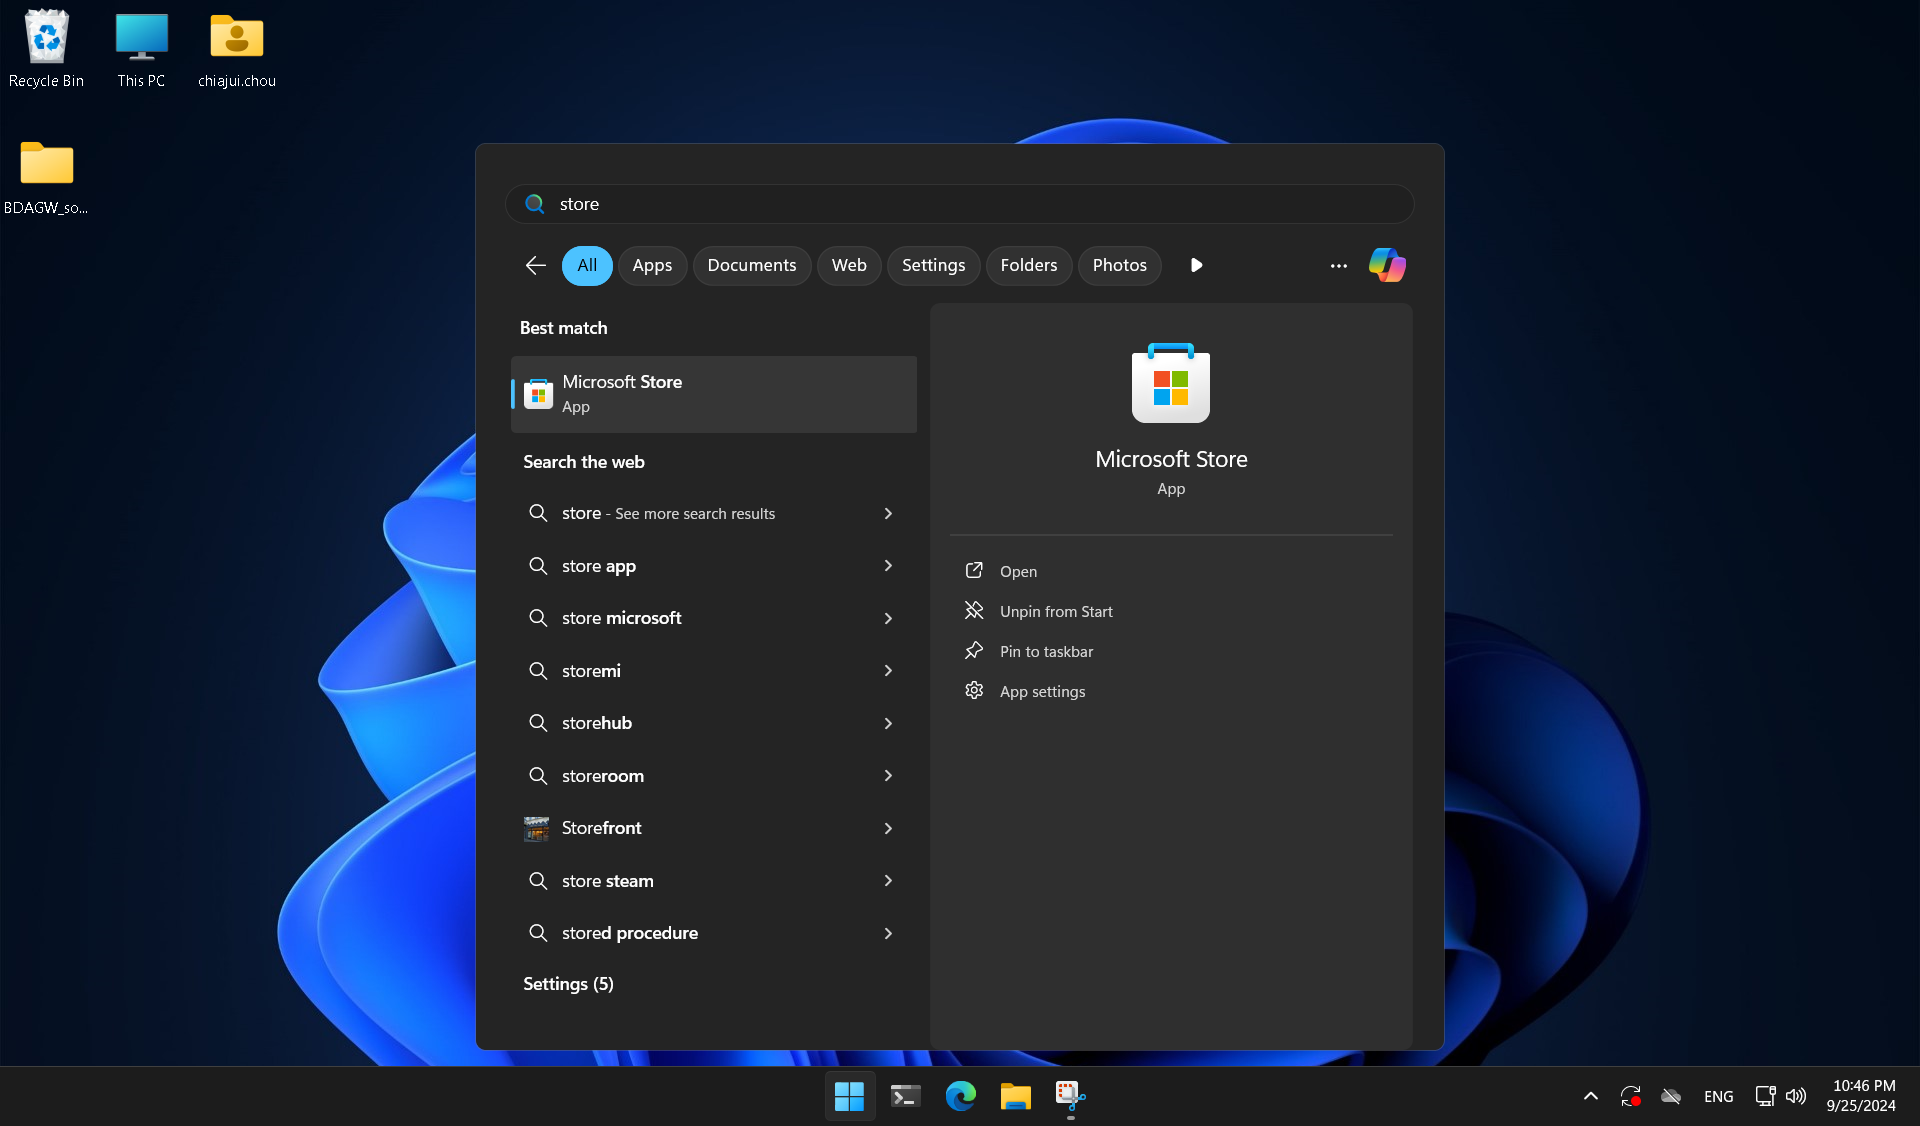
\includegraphics[width=\textwidth]{./image/microsoft_store}
        \caption{Microsoft Store}
    \end{subfigure}
    \begin{subfigure}[h]{0.48\textwidth}
        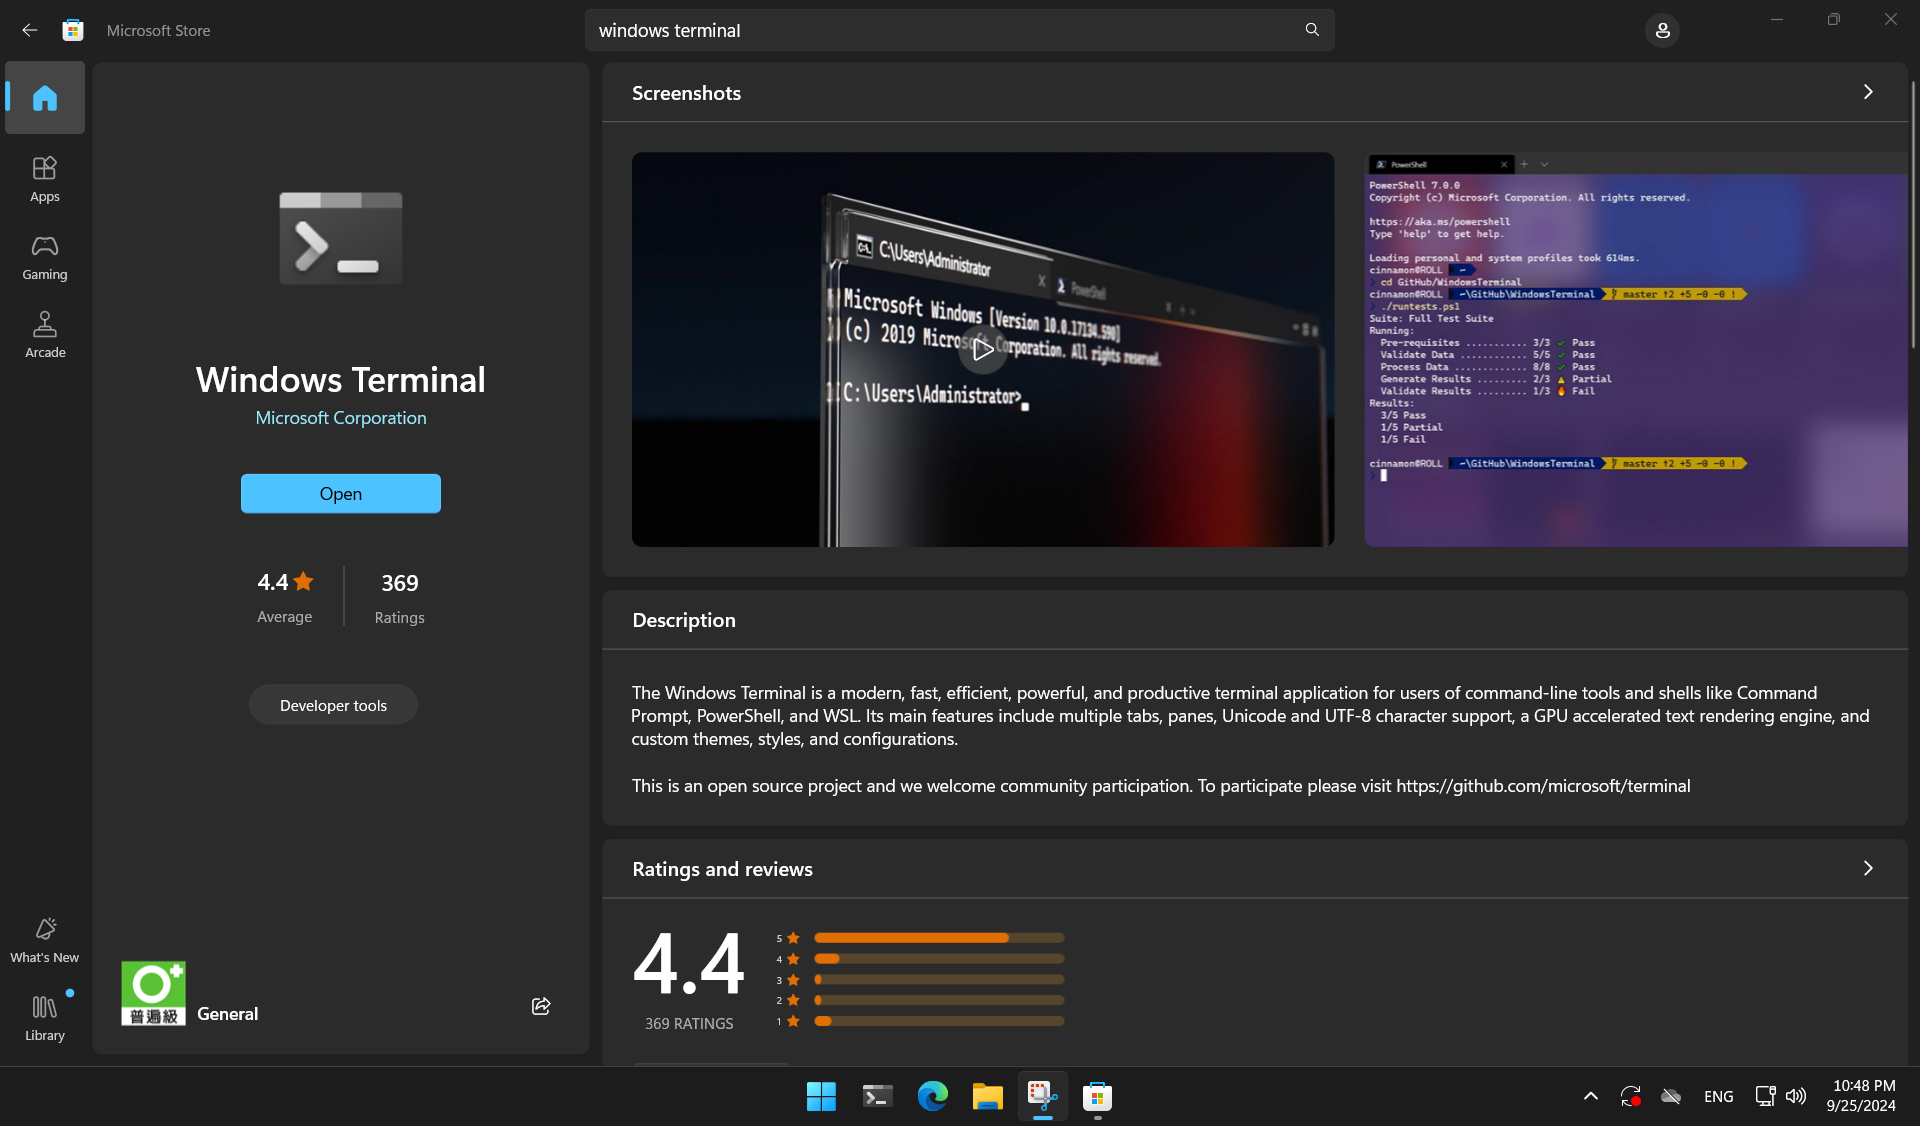
\includegraphics[width=\textwidth]{./image/install_windows_terminal}
        \caption{Install Windwos Terminal}
    \end{subfigure}
    \begin{subfigure}[h]{0.48\textwidth}
        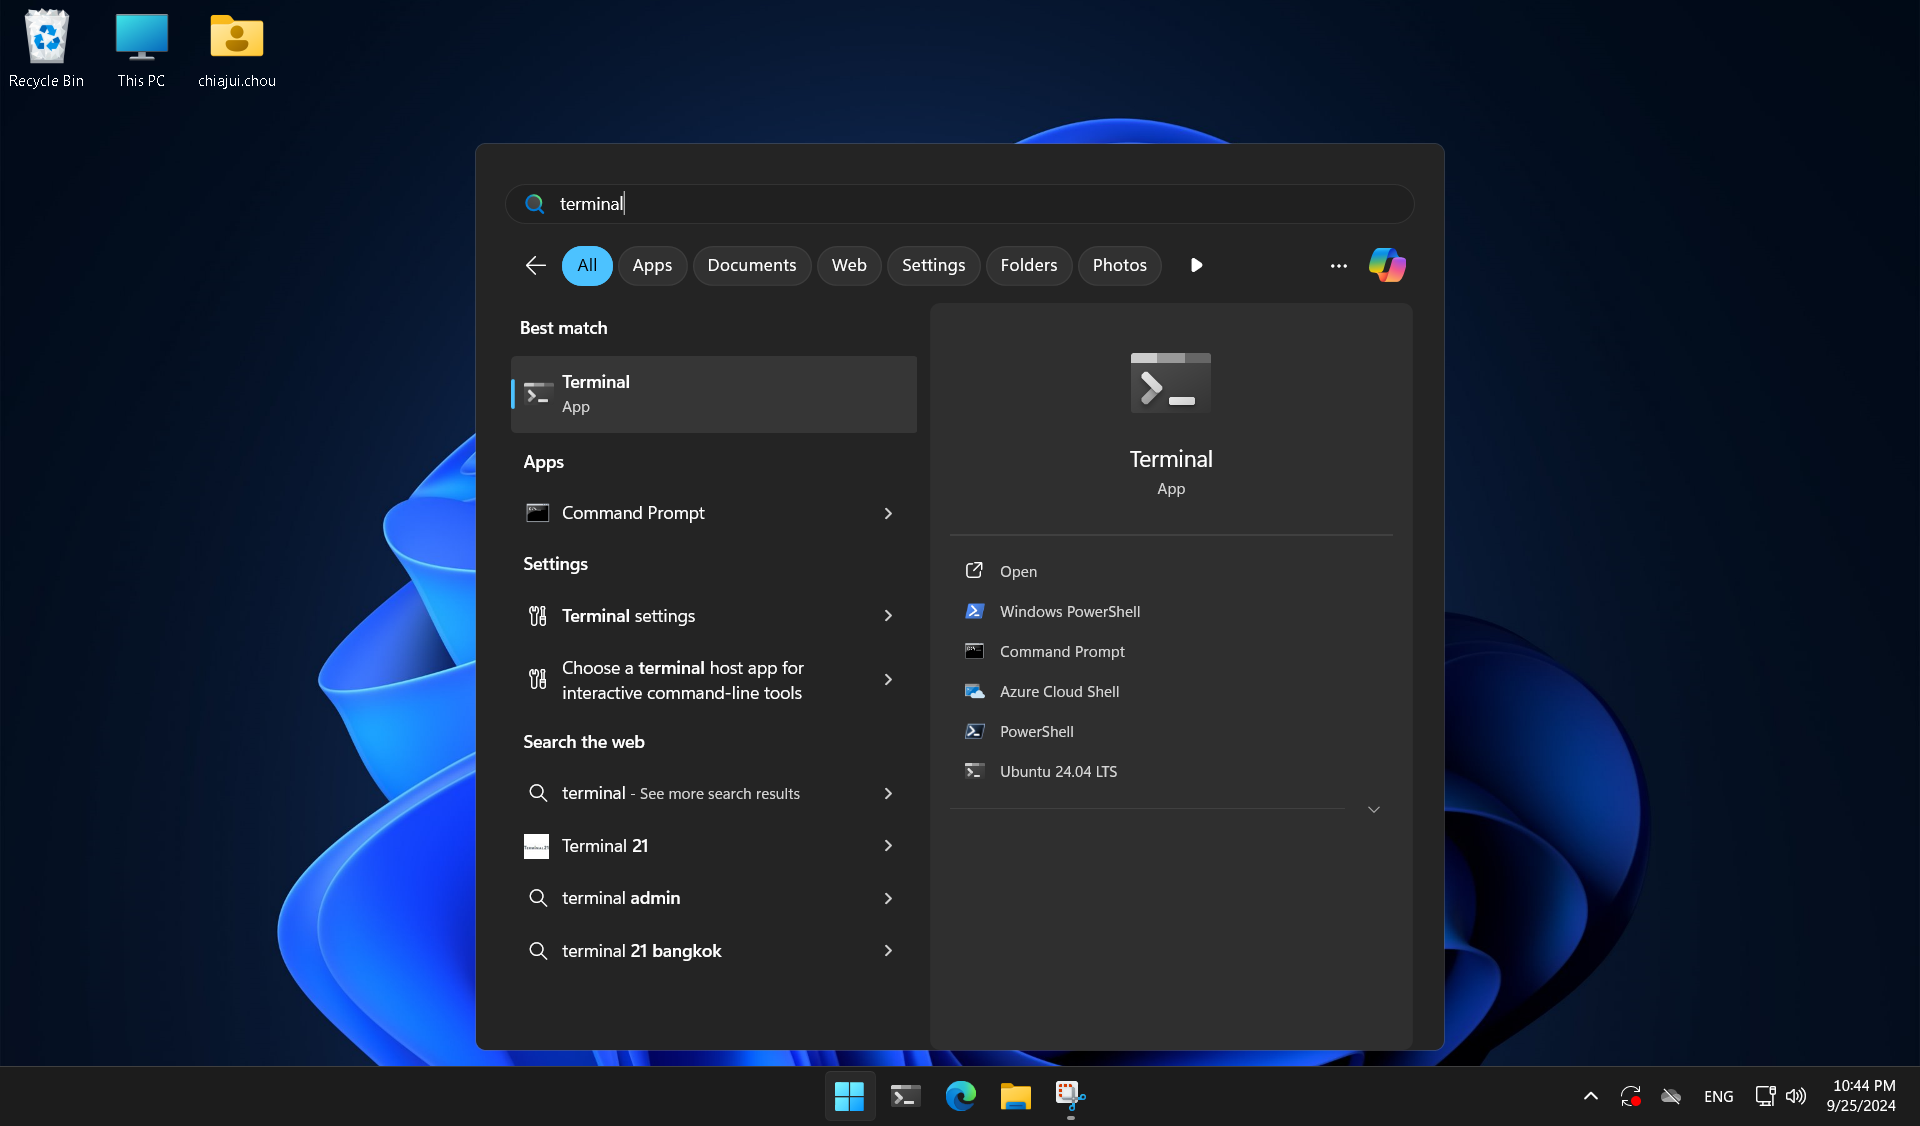
\includegraphics[width=\textwidth]{./image/windows_terminal}
        \caption{Launch Windows Terminal}
    \end{subfigure}
\end{figure}

%%%%%%%%%%%%%%%%
\subsection{Installing WSL 2}
References: 
\begin{enumerate}
    \item \href{https://learn.microsoft.com/en-us/windows/wsl/install}{\color{blue}\underline{https://learn.microsoft.com/en-us/windows/wsl/install}},
    \item \href{https://learn.microsoft.com/en-us/windows/wsl/install-manual}{\color{blue}\underline{https://learn.microsoft.com/en-us/windows/wsl/install-manual}}.
\end{enumerate}
Here are the steps to install the Linux subsystem under Windows 10/11:
\begin{enumerate}
    \item Enable the Windows Subsystem for Linux and the Virtual Machine feature:
    \begin{itemize}
        \item Open {\bf Control Panel $\rightarrow$ Uninstall a program $\rightarrow$ Turn Windows features on or off}.
        \item Check the following items (You can skip some of the items if you don't see it on your computer.):
        \begin{itemize}
        \item {\bf Hyper-V}
            \item {\bf Virtual Machine Platform}
            \item {\bf Windows Hypervisor Platform}
            \item {\bf Windows Subsystem for Linux}
        \end{itemize}
    \end{itemize}
    \item Install WSL 2 Linux kernel:
    \begin{itemize}
        \item Download the latest package from here: \href{https://wslstorestorage.blob.core.windows.net/wslblob/wsl_update_x64.msi}{\color{blue}\underline{here}} (this link can be found in {\bf Step 4} on the second reference).
        \item Update the Linux kernel by running the msi file.
        \item Reboot computer.
    \end{itemize}
    \item Set WSL 2 as default version:
    \begin{itemize}
        \item Open {\bf Windows Terminal}.
        \item Type the command in the terminal: \verb+wsl --set-default-version 2+ and press {\bf Enter key}.
    \end{itemize}
    \item Install a Linux distribution:
    \begin{itemize}
        \item Look for available Linux distributions:
        \begin{verbatim}
            wsl -l -o
        \end{verbatim}
        \item Install {\bf Ubuntu-22.04}:
        \begin{verbatim}
            wsl --install -d Ubuntu-22.04
        \end{verbatim}
        \item Launch WSL by \verb+wsl+ and set {\bf username} and {\bf password}.
        \item Check the distribution and version of the Linux system we install:
        \begin{Verbatim}[commandchars=\\\{\}]
            \home$ cat /etc/*release
        \end{Verbatim}
    \end{itemize}
\end{enumerate}
\newpage

%%%%%%%%%%%%%%%%
\subsection{Visual Studio Code}
It's recommanded to use Visual Studio Code as our Integrated Development Environment. You can follow the instructions here \href{https://code.visualstudio.com/}{\color{blue}\underline{https://code.visualstudio.com/}} to install Visual Stuido Code.

After installation, we need to install several extensions:
\begin{enumerate}
    \item Python
    \item Jupyter
    \item Remote Development
    \item WSL
\end{enumerate}
\begin{figure}[ht]
    \centering
    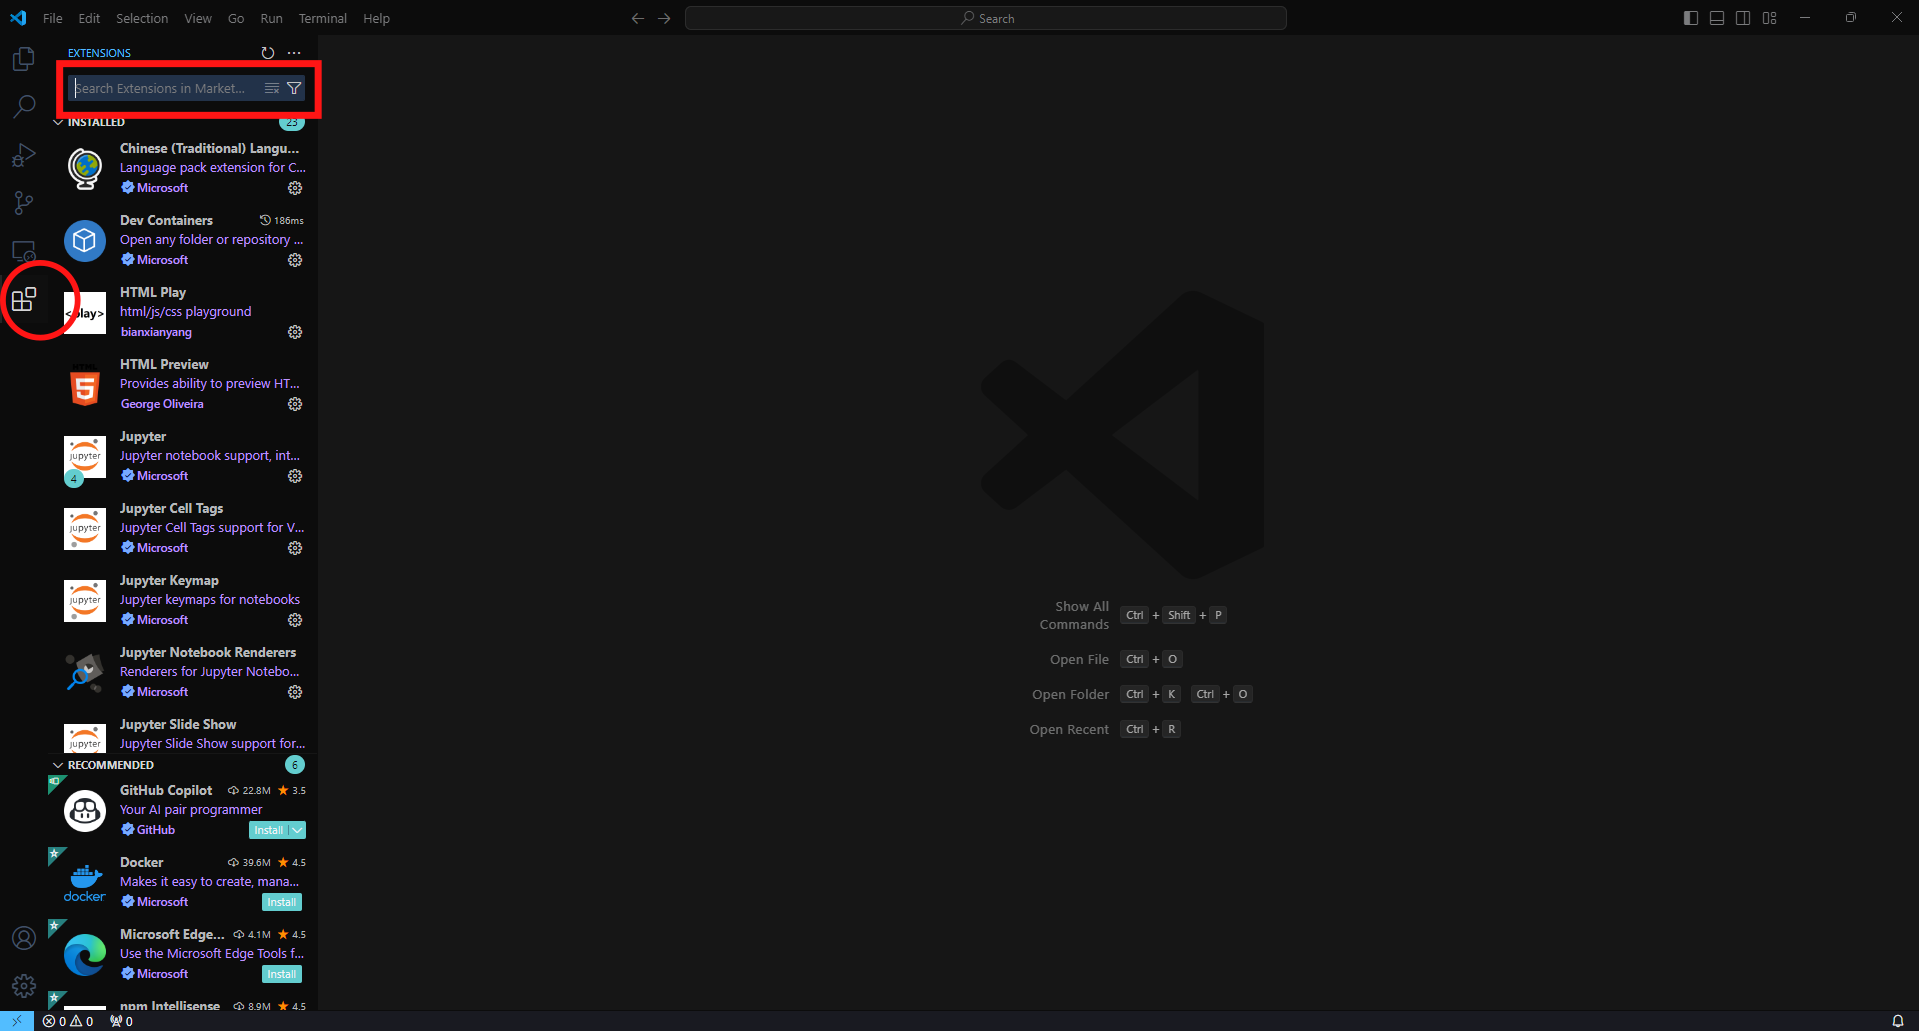
\includegraphics[width=0.8\textwidth]{./image/vscode-extensions.png}
    \caption{To install extensions, we click the extension icon and search for the extensions in the search bar.}
\end{figure}

%%%%%%%%%%%%%%%%
\subsection{Google Colab}
You can also use Google Colab \href{https://colab.research.google.com/}{\color{blue}\underline{https://colab.research.google.com/}} to edit and run jupyter notebooks.
